\newcommand{\var}{\mathrm{Var}}

    \problem
    \begin{question}
        Suppose that $f(t)$ is a continuous deterministic function
        such that $f'$ is square integrable, i.e., $\int_{\mathbb R}|f'(s)|^2ds<\infty$.
        Indeed this derivative could be understood in the ``weak sense" if this makes
        sense to you.  Prove that $f$ is of zero quadratic variation.
        This should give you an impression on the differences between the stochastic
        process $W_t$ and deterministic functions.
    \end{question}
    \begin{proof}
        Consider any interval $[a,b]$, then by definition the
        quadratic variation of $f$ is
        \[\lim_{N\to\infty}\sum_{i=0}^{N-1} (f(x_{i+1})-f(x_i))^2\]
        where $a=x_0<x_1<\cdots<x_N=b$ is a partition of $[a,b]$.
        Since $f$ is differentiable on $\mathbb R$, then by mean
        value theorem, we have that
        \[f(x_{i+1})-f(x_i)=f'(\xi_i)(x_{i+1}-x_i)\]
        where $x_i\leq \xi_i\leq x_{i+1}$.
        If we denote $\tau=\max_{0\leq i\leq N}(x_{i+1}-x_i)$,
        then we have that
        \[\begin{aligned}
            \sum_{i=0}^{N-1}(f(x_{i+1})-f(x_i))^2
            &=\sum_{i=0}^{N-1}(f'(\xi_i))^2(x_{i+1}-x_i)^2\\
            &\leq\tau\sum_{i=0}^{N-1}(f'(\xi_i))^2(x_{i+1}-x_i)
        \end{aligned}\]

        Also we know that $f'^2$ is integrable on $\mathbb R$
        thus the subinterval $[a,b]$, namely
        \[\int_a^b|f'(\xi)|^2\diff\xi<\infty\]
        hence for the partition above, by definition of Riemann
        integral the following limit exists
        \[\lim_{N\to\infty}\sum_{i=0}^N(f'(\xi))^2(x_{i+1}-x_i)
        <\infty\]
        It follows that
        \[\lim_{N\to\infty}\tau\sum_{i=0}^N(f'(\xi))^2(x_{i+1}-x_i)
        =0\]
        as $N\to\infty$ means $\tau\to 0^+$. Therefore
        \[\sum_{i=0}^N(f(x_{i+1})-f(x_i))^2\to 0\]
        as $N\to\infty$, i.e., the quadratic variation on $[a,b]$
        is 0, and by the arbitrariness of $a,b$, this entity holds
        on $\mathbb R$.
    \end{proof}

    \problem
    \begin{question}
    Let us denote as in class 
    \[R_N:=\sum^{N-1}_{i=0}\Delta Z_i(W_{t_{i+1}}-W_{t_{i}})\]
    with 
    \[\Delta Z_i=(W_{t^*_{i}}-W_{t_{i}})-(W_{t_{i+1}}-W_{t^*_{i}}), t^*_i=\frac{t_i+t_{i+1}}{2}.\]
    Prove that m.s.-$R_N\rightarrow 0$ as $N\rightarrow \infty$.
    \end{question}
    \begin{proof}
        Since
        \[\begin{aligned}
            R_N&=\sum_{i=0}^{N-1}\Delta Z_i(W_{t_{i+1}}-W_{t_i})\\
            &=\sum_{i=0}^{N-1}\big(2W_{t_i^*}-(W_{t_{i_1}}+W_{t_i})
              \big)(W_{t_{i+1}}-W_{t_i})\\ 
            &=2\sum_{i=0}^{N-1}W_{t^*_i}(W_{t_{i+1}}-W_{t_i})
              -\sum_{i=0}^{N-1}(W_{t_{i+1}}^2-W_{t_i}^2)\\
        \end{aligned}\]
        of which the fisrt term is the Stratonovich integral\sidenote{%
        It is a Riemann sum of Stratonovich integral,
        to be more rigorous.}, namely,
        \[\sum_{i=0}^{N-1}W_{t_i^*}(W_{t_{i+1}}-W_{t_i})\to\frac{W_T^2}{2}
        \text{ m.s. }(N\to\infty)\]
        then we have that
        \[R_N\to 0\text{ m.s.}\]
        as
        \[\sum_{i=0}^{N-1}(W_{t_{i+1}}^2-W_{t_i}^2)=W_T^2-W_0^2=W_T^2\]
    \end{proof}

    \problem
    \begin{question}
        Let us recall that the stochastic integral is defined as the mean square
        limit of finite sum, whence an concrete example shows
        \[\int_0^T f(\omega,t)dW_t=\text{m.s.}-\lim_{N\rightarrow\infty}
        \sum^{N-1}_{i=0}\Delta f(\omega,t^*_i)(W_{t_{i+1}}-W_{t_{i}}).\]
        Here the choice $t^*_i=t_i$ leads to the It\^o, $t^*_i=\frac{t_{i+1}+t_{i}}{2}$
        the Stratonovich integral.  As I mentioned in class, by default an integral
        with respect to a stochastic process is defined as the It\^o.

        Let us consider the general choice $t^*_i=(1-\lambda)t_i+\lambda t_{i+1}$,
        with an arbitrary but fixed $\lambda\in[0,1]$.  Find the following limit
        (I used the diamond for a generic notation)
        \[\int_0^T W_t \diamond dW_t=\text{m.s.}-\lim_{N\rightarrow\infty}\sum^{N-1}_{i=0} W_{t^*_i}(W_{t_{i+1}}-W_{t_{i}}).\]
        We collect the It\^o when $\lambda=0$ and the Stratonovich when
        $\lambda=\frac{1}{2}$, therefore your result should recover theirs. 
    \end{question}
    Denote
    \[I_N=\sum_{i=0}^{N-1}W_{t_i^*}(W_{t_{i+1}}-W_{t_i})\]
    then to avoid the overlap between interval $[0,t_i^*]$ and $[t_i,t_{i+1}]$
    for independence consideration, do the decomposition,
    \[\begin{aligned}
        I_N&=\sum_{i=0}^{N-1}W_{t_i^*}(W_{t_{i+1}}-W_{t_i^*})
        +W_{t_i^*}(W_{t_i^*}-W_{t_i})\\
    \end{aligned}\]
    and we split $W_{t_i^*}$ again in the last term,
    \[\begin{aligned}
        I_N&=\sum_{i=0}^{N-1}W_{t_i^*}(W_{t_{i+1}}-W_{t_i^*})
        +(W_{t_i^*}-W_{t_i})^2+W_{t_i}(W_{t_i^*}-W_{t_i})\\
        &=\sum_{i=0}^{N-1}\left(W_{t_i^*}(W_{t_{i+1}}-W_{t_i^*})
            +W_{t_i}(W_{t_i^*}-W_{t_i})\right)
          +\sum_{i=0}^{N-1}(W_{t_i^*}-W_{t_i})^2
    \end{aligned}\]
    Now take a close look at the first term, and it is easy to
    see that it is the It\^o  integral actually, i.e., consider
    the following partition\sidenote{If $\lambda=0\text{ or }1$,
    then it is not a partition. But it is a degenerated case actually,
    namely a partition with $N$ slices, so it is ok as well.} of $[0,T]$,
    \[0=t_0<t_0^*<t_1<t_1^*<\cdots<t_{N-1}<t_{N-1}^*<t_N=T\]
    and denote 
    \[\tilde t_i=\begin{cases}
        t_k&,i=2k\\
        t_k^*&,i=2k+1
    \end{cases}\]
    then $0=\tilde t_0<\tilde t_1<\cdots<\tilde t_{2N}=T$ is the finer
    partition, thus
    \[\sum_{i=0}^{N-1}\left(W_{t_i^*}(W_{t_{i+1}}-W_{t_i^*})
            +W_{t_i}(W_{t_i^*}-W_{t_i})\right)
    =\sum_{i=0}^{2N}W_{\tilde t_i}(W_{\tilde t_{i+1}}-W_{\tilde t_i})\]
    which will converge to $(W_T^2-T)/2$ in m.s. as we leant
    in class.

    As for the latter term, we obtained its variance as
    \[\var\left(\sum_{i=0}^{N-1}(W_{t_i^*}-W_{t_i})^2\right)
    =\sum_{i=0}^{N-1}\var\left((W_{t_i^*}-W_{t_i})^2\right)
    =\sum_{i=0}^{N-1}2(t_i^*-t_i)^2\]
    by the independence of each term and formula,
    \[\var(X^2)=2\sigma^4\text{ if }X\sim\mathcal N(\mu,\sigma^2)\]
    If we denote $\tau=\sup_{0\leq i\leq N-1}(t_{i+1}-t_i)$ to describe
    the mesh, then $N\to\infty$ is equivalent to $\tau\to 0^+$, and
    \[\begin{aligned}
        \var\left(\sum_{i=0}^{N-1}(W_{t_i^*}-W_{t_i})^2\right)
    &\leq 2\sum_{i=0}^{N-1}(t_{i+1}-t_i)^2\\
    &\leq 2\tau\sum_{i=0}^{N-1}t_{i+1}-t_i\\
    &=2T\tau\to 0\quad(\tau\to 0^+)
    \end{aligned}\]
    and the expectation
    \[\begin{aligned}
        E\left(\sum_{i=0}^{N-1}(W_{t_i^*}-W_{t_i})^2\right)
        &=\sum_{i=0}^{N-1}t_i^*-t_i\\
        &=\sum_{i=0}^{N-1}(1-\lambda)t_i+\lambda t_{i+1}-t_i\\
        &=\lambda\sum_{i=0}^{N-1}t_{i+1}-t_{i}\\
        &=\lambda T
    \end{aligned}\]
    therefore,
    \[\sum_{i=0}^{N-1}(W_{t_i^*}-W_{t_i})^2\to\lambda T
    \text{ in m.s.}\]
    It follows that
    \[I_N\to \frac{W_T^2}{2}+\left(\lambda-\frac{1}{2}\right)T
    \quad(N\to\infty)\]
    in m.s., i.e.,
    \[\int_0^TW_t\diamond\diff W_t=
    \frac{W_T^2}{2}+\left(\lambda-\frac{1}{2}\right)T\]

    \problem
    \begin{question}
        Similar as the Riemann-Stieljes integral, one can define an integral not only against
        a Brownian but any stochastic processes $X_t$ as follows, provided the result is well
        and properly defined
        \[\int_0^T f(\omega,t)dX_t=\text{m.s.}-\lim_{N\rightarrow\infty}\sum^{N-1}_{i=0}
        \Delta f(\omega,t^*_i)(X_{t_{i+1}}-X_{t_{i}}).\]
        Use definition to find 
        \[\int_0^T s d(W^2_s).\]
        You can also try to evaluate $\int_0^T s d(W^3_s)$, and $\int_0^T W_s d(W^3_s)$
        by bare hand, but one will find that the calculations can be challenging and tedious
        if merely by brutal forces.  Therefore they call for user-friendly formulas that we
        shall introduce later in this course.
    \end{question}
    By definition,
    \[\int_0^Ts\diff(W_s^2)
    =\lim_{N\to\infty}I_N
    =\lim_{N\to\infty}\sum_{i=0}^{N-1}t_i^*(W_{t_{i+1}}^2-W_{t_i}^2)\]
    where\sidenote{Again $t^*_i$ should be in $[t_i,t_{i+1}]$ exactly,
    i.e., it can achieve both ends.
    but it doesn't matter in my opinion, and strict inequality makes
    the following analysis more clear.}
    $0=t_0<t_0^*<t_1<t_1^*<\cdots<t_{N-1}<t_{N-1}^*<t_N=T$.
    Note that the discrete term
    \[\begin{aligned}
        t_0^*(W_{t_1}^2-W_{t_0}^2)&=t_0^*W_{t_1}^2-t_0^*W_{t_0}^2\\
        t_1^*(W_{t_2}^2-W_{t_1}^2)&=t_1^*W_{t_2}^2-t_1^*W_{t_1}^2\\
        t_2^*(W_{t_3}^2-W_{t_2}^2)&=t_2^*W_{t_3}^2-t_2^*W_{t_2}^2\\
        &\cdots\\
        t_{N-1}^*(W_{t_N}^2-W_{t_{N-1}}^2)&=t_{N-1}^*W_{t_N}^2-t_{N-1}^*W_{t_{N-1}}^2\\
    \end{aligned}\]
    hence
    \[\begin{aligned}
        I_N
        &=t_{N-1}^*W_{t_N}^2-t_0^*W_{t_0}^2
          +\sum_{i=0}^{N-2}(t_i^*-t_{i+1}^*)W_{t_{i+1}}^2\\
        &=t^*_{N-1}W_T^2
          +\sum_{i=0}^{N-2}(t_i^*-t_{i+1}^*)W_{t_{i+1}}^2\\
    \end{aligned}\]
    where the last term is stochastical process integral
    over time, which we will see next.

    For any $\omega\in\Omega$, by definition\sidenote{The reason
    why the last term looks so weird is that there is no $t^*_N$
    and we omitted the first term which is 0.}
    \[\int_0^TW_t^2\diff t
    =\lim_{N\to\infty}\left(\sum_{i=0}^{N-2}W_{t_{i+1}}^2(t^*_{t+1}-t^*_i)
    +W_T^2(T-t_{N-1}^*)\right)\]
    where we chosed a partition
    $0<t_0^*<t_1^*<t_2^*<\cdots<t_{N-1}^*<T$ and
    sample point $t_i\in(t_{i-1}^*,t_i^*)$
    (the first and last sample point is $0$ and $T$
    accordingly).
    It following that
    \[\lim_{N\to\infty}(TW_T^2-I_N)
    =\int_0^TW_t^2\diff t\]
    pointwisely.
    Therefore
    \[\lim_{N\to\infty}I_N
    =TW_T^2-\int_0^TW_t^2\diff t\]
    pointwisely. In other word\sidenote{So I just converted
    a stochastic integral to another random variable which
    may be complex as well.
    And this seems to be a trival result of integral by parts.
    But I still can't find a traditional
    way to calculate this integral in the m.s. sense as
    you showed in class.},
    \[\int_0^Ts\diff(W_s^2)=TW_T^2-\int_0^TW_s^2\diff s\]



    \problem
    \begin{question}
        We will show later in this course that the following differential equation
        with $\mu,\sigma\in\mathbb R$
        \begin{equation}\label{GBM}
        dX_t=\mu X_tdt+\sigma X_tdW_t, t>0, X_0=x_0\in\mathbb R.
        \end{equation}
        admits a unique and explicit solution: the GBM
        $X_t=x_0\exp\{(\mu-\frac{\sigma^2}{2})t+\sigma W_t\}$.

        We are not motivated to solve this equation analytically but numerically.
        To this end, let us integrate (\ref{GBM}) over $(0,T)$, and then
        one naturally have that
        \begin{equation}\label{int}
        X_T-x_0=\int_0^T\Big(\mu X_tdt+\sigma X_tdW_t\Big)=\mu \int_0^TX_tdt+\sigma  \int_0^T X_tdW_t.
        \end{equation}
        One can easily prove why the identities holds for the Riemann integral,
        and indeed they also hold for the stochastic ones though we do not verify
        them here rigorously.

        According to (\ref{int}), solving for $X_t$ becomes evaluating the integrals
        therein, and numerically this can only done iteratively since the explicit
        formula of $X_t$ is not available.  We integrate (\ref{GBM}) over
        $(k\Delta t,(k+1)\Delta t)$ for $\Delta t$ sufficiently small.  Therefore
        \begin{fullwidth}
        \[X_{(k+1)\Delta t}-X_{k\Delta t}=\mu \int_{k\Delta t}^{(k+1)\Delta t}X_tdt
        +\sigma  \int_{k\Delta t}^{(k+1)\Delta t} X_tdW_t\approx \mu X_{k\Delta t}\Delta t
        +\sigma X_{k\Delta t}(W_{(k+1)\Delta t}-W_{k\Delta t}),\]
        \end{fullwidth}
        and we use the equation
        \[X_{(k+1)\Delta t}= X_{k\Delta t}+\mu X_{k\Delta t}\Delta t
        +\sigma X_{k\Delta t}(W_{(k+1)\Delta t}-W_{k\Delta t}),\]
        starting with $X_0=x_0$, with each $k\in\mathbb N^+$, as an approximation
        of $X_t$ should $\Delta t$ be chosen properly small.
        Here $W_{(k+1)\Delta t}-W_{k\Delta t}$ is a Brownian motion that we numerically
        introduced last homework.  This is an analogy of the forward Euler's method for ODEs.
        Iterating this difference equation to $T/\Delta t$ steps leads to an approximation
        of the solutions.  I would like to elaborate that the discretization also gives us
        a strong motivation why the left end-point should be chosen here once the forward
        method is favored.  Plot the solution for $T=1$, $\mu=0.1$, $\sigma=2$ with $X_0=1$.
        Needless to say, the solution $X_T$ is a stochastic process, therefore what
        you plotted is a (realized) sample path of the solution.
    \end{question}
    See \cref{fig:numerical solution}.
    \begin{figure}[h]
        \centering
        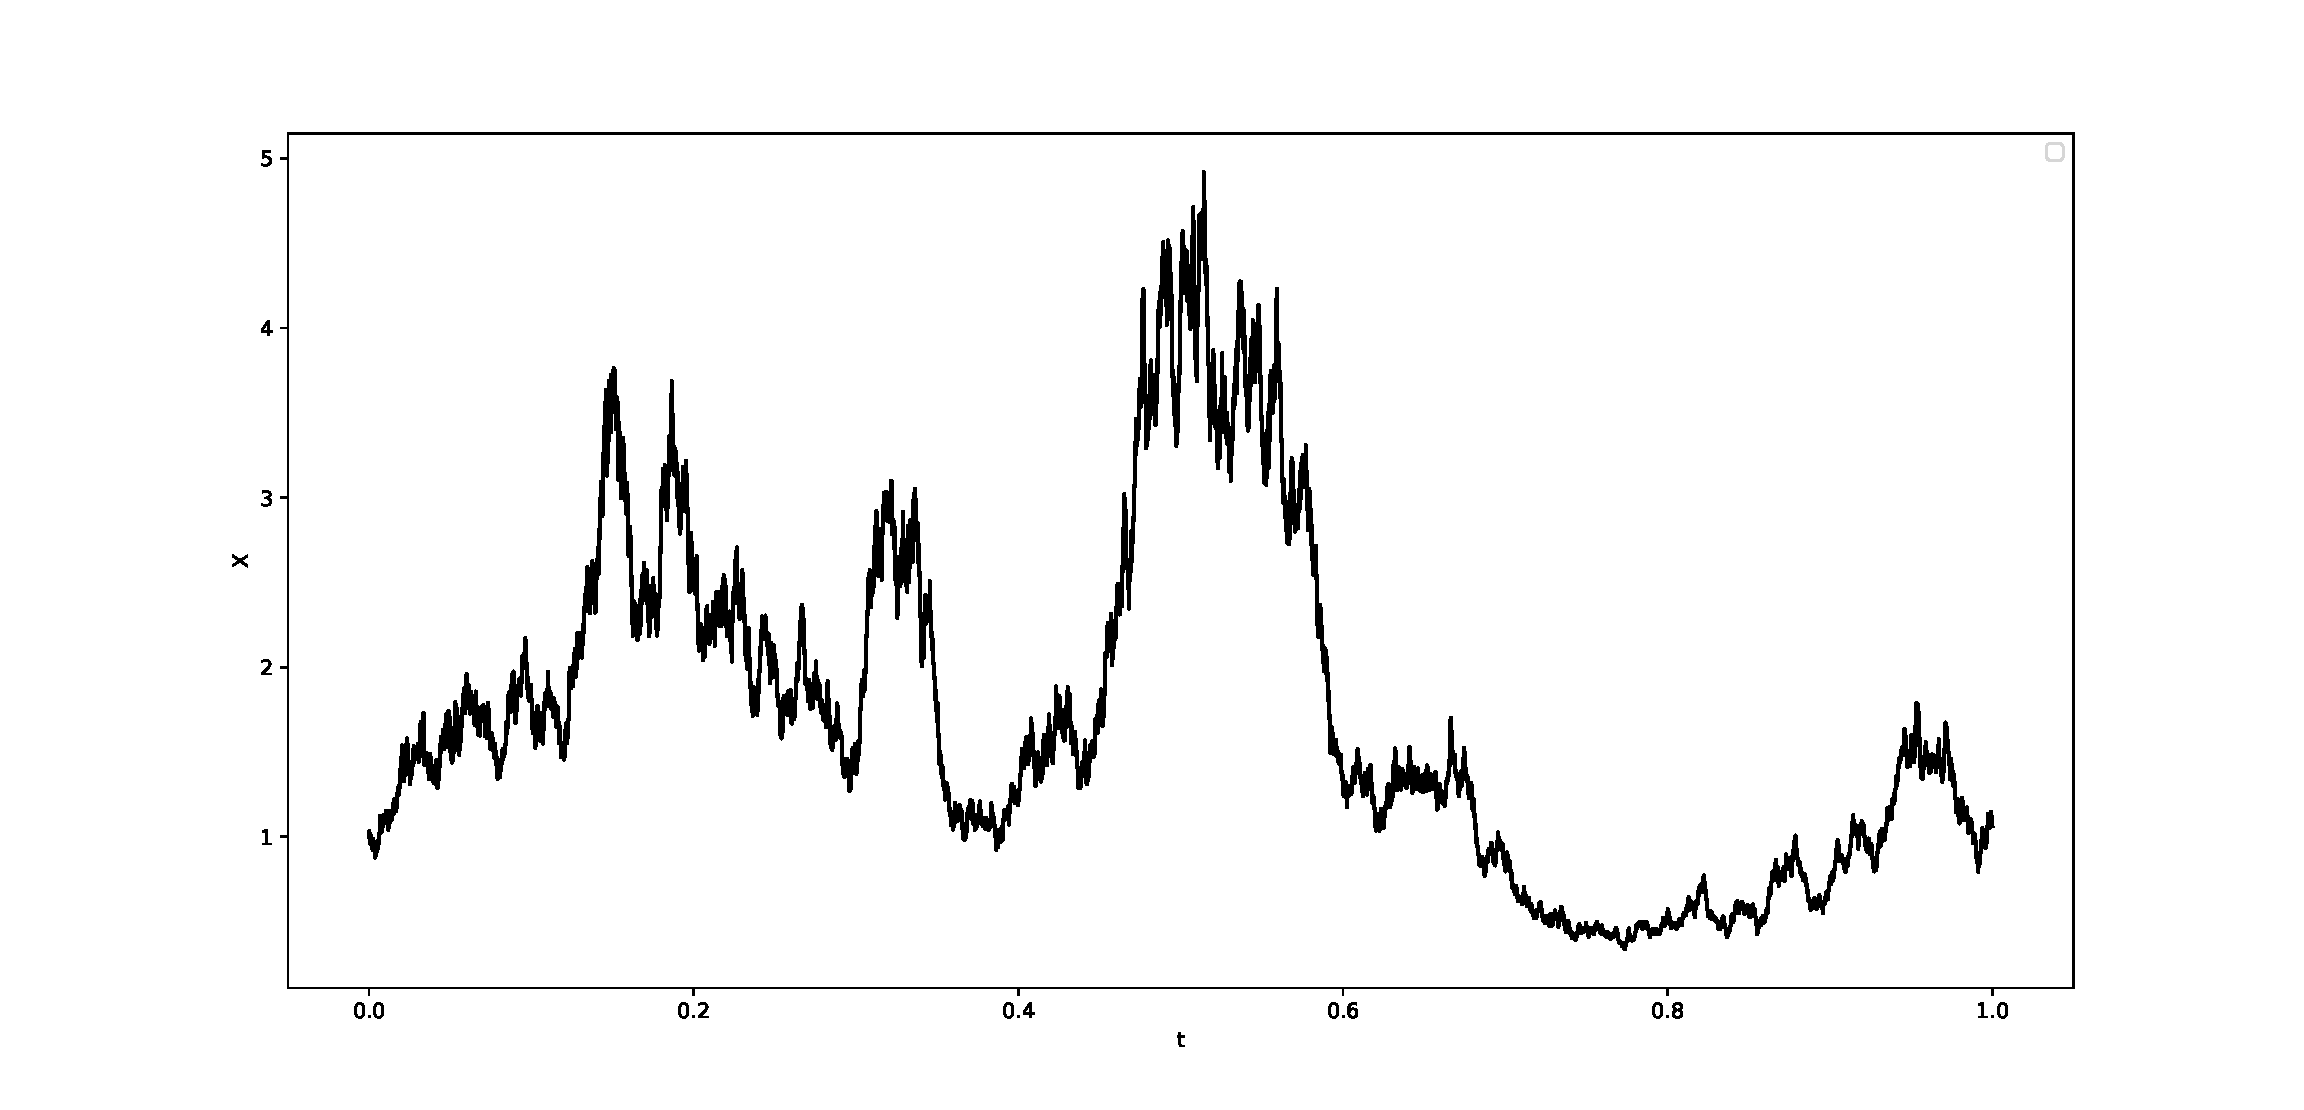
\includegraphics[width=\linewidth]{solution}
        \caption{Numerical Solution}
        \label{fig:numerical solution}
    \end{figure}

    \appendix
    \section{Python Code for Numerical Solution}
    \lstinputlisting[language=Python]{numerical.py}